\chapter{Solving Einstein Equations}

While studying gravitational collapse of a scalar field we got a set of differential equations. These differential equations were complicated enough that any effort to find an analytical solution was futile. One can always make some approximations and get some understanding of the solutions, but to get a complete solution we need to use numerical techniques. In this chapter we will discuss about how to solve differential equations on a computer.




\section{Finite difference methods}

Solving differential equations is required in almost every field of Science and although analytical solution are the best thing one can get, they are hard to come by.
Most of the time we have to resort to solving differential equation numerically. There a lot of methods out there developed to solve differential equations, each of them have their own advantages and dis-advantages. In our case we will be using a class of methods called finite difference methods.

\index{Finite difference methods} Finite difference methods are the most intuitive and easy to implement methods. They are derived using the taylor series and give a discrete approximation of the strong from of the differential equations.

To get some intuition about finite difference methods let us start with a very simple example. These simple examples will demonstrate some of the most important concepts of finite difference computing.

Suppose that we want to find the value of the derivative of the function $f(x) = x^3$ at $x =1$. We know that the answer should be $3$. But, let us say that we do not know the exact formula and want to approximate the derivative.
The simplest way to do this would be using the formula of the derivative itself,

\begin{equation}
    \frac{dy(x_0)}{dx} = \lim_{h \to 0}\frac{y(x_0 + h) - y(x_0)}{h}
\end{equation}

The definition of derivative gives us the exact answer in the limit. What we can do is to take $h$ to a small non-zero number and see if that gives us an approximate answer.

\begin{equation}
    \frac{dy(x_0)}{dx} \approx \frac{y(x_0 + h) - y(x_0)}{h} , \text{for } h << 1
\end{equation}\label{eq:first_order}

We have shown the results of using the equation \ref{eq:first_order} to approximate the derivative of $x^3$ at $x=1$ in the figure \ref{fig:x^3_error_order1}. Y axis in the figure is the log error of the approximation and X axis is the log of the \index{step size} step size ($h$). Figure \ref{fig:x^3_error_order1} has a lot of stuff going on in it and we will break it down into parts. But before we do that we will briefly look at how computers store decimal numbers and how does it affect our calculations.

\subsection{Floating point arithmetic}

\index{Floats} Floats are how computers internally represent decimal numbers. A larger sized float can handel both a larger number and more significant digits\index{significant digits}. Because computers can only stores a fixed number of digits after the decimal point we get \index{floating point errors} floating point errors whenever any calculation is done on these floats. For example we know that $\frac{1}{3}$ has a recurring decimal expansion, but if we want to save $\frac{1}{3}$ in the computer, in its decimal representation, then there will be a small error because we can only store a fixed number of significant digits.




\begin{table}[hbt!]
    \centering
    \begin{tabular}{||m{2cm} | m{3.2cm} | m{1.5cm} | m{4.5cm}||}
        \hline
        Float type & Largest Number that can be stored* & Precision & How is $\frac{1}{3}$ internally stored \\ [0.5ex]
        \hline\hline

        Float32    & 3.40e+38                           & 6         & 0.33333334                             \\

        Float64    & 1.79e+308                          & 15        & 0.3333333333333333                     \\

        Float128   & 3.36e+4932                         & 18        & 0.33333333333333333334                 \\ [1ex]
        \hline
    \end{tabular}
    \caption{This table shows the largest number that can be represented by a particular type of float (* rounded off to two decimal places). Precision denotes the number of significant decimal digits that can be represented by a float type.}
    \label{table:floats}
\end{table}

Table \ref{table:floats} has the information about different kind of floats used in the graphs. \index{Precision}Precision denotes the number of significant digits that a particular type of float can store, for example, float32 can store just 6 numbers after the decimal point which is why $\frac{1}{3}$ is stored as $0.33333334$. Also, note that the there is a huge difference in the largest number that can be stored between different kind of floats. If we try to store a number larger than the maximum number that a float type can hold we get an overflow error and computer starts giving us random garbage. Different languages and libraries deal with such errors in different ways and it is not worth going into the specifics, but the bottom line is that we can not work with float64 if our systems have numbers larger than $1.79*10^{308}$.


Most of the modern computers chips use float64 internally and they have CPU circuits that are very efficient in working with float64 numbers. Float64 denotes that this number will use 64bits of memory, while float32 numbers only use 32bits of memory; this means that we can store more float64 numbers in the same amount of memory. What this means in practical terms is that a we can store around $10^9$ floats in $8GB$ of RAM, or a matrix with approximately 31000 rows and columns. If we are not clever with what we are storing in our RAM there is real danger that we may run out of memory, which will cause an error and our program will stop.


Among the parameters listed in Table \ref{table:floats} the most important parameter for any calculation is the precision. As already mentioned whenever we perform any kind of operation on a floating point number there is an error due to the \index{finite precision}finite precision of floating point numbers.
We can see this phenomenon quite easily just by adding $1.0$ to $\frac{1}{3}$ stored as a float32. If we add $1.0$ to $0.\overline{33}$, $10000$ times the expected answer is $10000.\overline{33}$ which in float32 precision should be $10000.3333334$. But, we see that the actual answer that we get is $10000.334$, that is we have lost 4 significant digits.
This loss of accuracy is what we call \index{floating point error}floating point error and this is the reason why using float32 for numerical computations is a bad idea. If we use float64 instead of float32 we will still lose 4 significant digits but it will not so much because we will still have 11 significant digits in the decimal to work with. We should mention here that there is no hard and fast formula for how many digits will we lose per operation and it depends on the language and libraries used as many of them are optimized to reduce floating point errors.\label{para:addition_errors}

We will discuss one final point we need to discuss before we wrap up this section and go back to developing finite difference algorithms. Given any two floating point numbers, we want to ask that when are they equal to each other?
This question is important because it is related to the precision of floating point numbers. For example, if we try to subtract $1.0000001$ from $1.0000007$ and they are stored as float32, then we will get some random garbage. The reason being that float32 can not handle more than 6 decimal significant digits properly.
The general rule is that one should try to avoid subtracting two numbers that are close and have a lot of significant digits in their \index{mantissa}mantissa, as that usually gives a lot of error.
Just for the sake of clarity, we should mention that here we are not taking about numbers with small magnitude. So, even float32 can easily handle numbers of small magnitude like subtracting $2*10^{-30}$ from $1*10^{-30}$ because their mantissa does not have a lot of significant digits. But, at the same time $2 + 10^{-8}$ and $2$ will both be stores as $2.0$ inside the computer memory and will give zero if subtracted from each other.


Here we have given all the examples in float32 but the concepts carry over to float64, the only difference being that float64 can handle much smaller number and more significant digits. As already mentioned modern computers CPU's are designed to deal with float64 arithmetic and it is accurate enough so we use it for most of our calculations. Using float128 or larger floats can give much more accuracy but they will very slow compared to using float64 and are not required for most of the applications.

\subsection{Floating point errors in finite difference approximations}

Now that we have some idea about the floating point arithmetic we can dive into the graphs.
In the figure \ref{fig:x^3_error_order1} there are three lines, each corresponding to a different sized float used for the calculations.

To approximate the derivative of $x^3$ at $x=1$ we have used the formula,

\begin{equation}
    \frac{dy(x_0)}{dx} \approx \frac{y(x_0 + h) - y(x_0)}{h} , \text{for } h << 1
\end{equation}\label{eq:first_order_2}

This is called a \index{first order} first order finite difference approximation. To understand why is it called we will taylor expand the $y(x)$ around $x_0$ with step size $h$

\begin{equation}
    y(x_0 + h) = y(x_0) + y'(x_0)*h +\frac{y''(x_0)*h^2}{2} + \dots
\end{equation}

If we truncate the series at $O(h^2)$ and rearrange a little we get,

\begin{equation}
    y(x_0 + h) - y(x_0) \approx y'(x_0)*h +\frac{y''(x_0)*h^2}{2}
\end{equation}

dividing by $h$ we get,

\begin{equation}
    y'(x_0)  \approx \frac{y(x_0 + h) - y(x_0)}{h} - \frac{y''(x_0)*h}{2}
\end{equation}\label{eq:1d_1o_error}

Notice that this is the exact formula that we were using for approximating the derivative except for the presence of the extra term $\frac{y''(x_0)*h}{2}$. This extra term represents the error in our approximation (there are of course other higher order terms that we ignored, but this term is going to dominate them anyways). Because the error falls off with the step size $h$ we call this a first order approximation. Looking at the figure \ref{fig:x^3_error_order1} this becomes clear, if the step size was decreased by a factor of two then the error will also go down by a factor of two, i.e. slope of the log(error) vs log(h) line will have a slope 1.

\begin{figure}[hbt!]
    \centering
    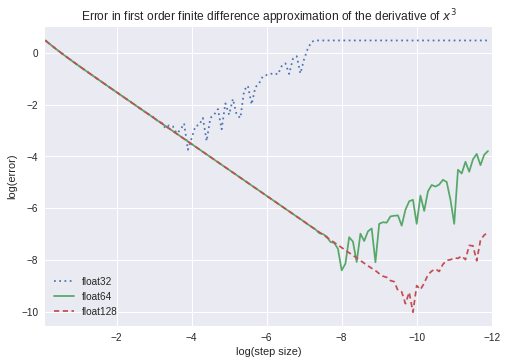
\includegraphics[width=\textwidth]{images/x^3_error_order1.png}
    \caption{This plot show error of using finite difference to approximate the derivative of $x^3$ vs the step size. Observe that the error falls almost linearly until the floating point errors start to dominate, after which it starts to grow erratically. Also, observe that for reasonable step sizes the error falls with a slope of 1, which is why such approximations are called to be of first order. }\label{fig:x^3_error_order1}
    \index{figures}
\end{figure}

In the beginning, irrespective of the float size, we have a straight line which turns into a wiggly mess as we keep on decreasing the step size. The reason for this sudden increase in the error is floating point errors. One can clearly see that going form float32 to float64 is a big jump in accuracy. But going to float128 from float64 the increase in the accuracy is not so dramatic, which is kind of expected as float128 has only 3 more significant digits over float64.

We can also use higher order methods, for example a second order method,

\begin{equation}
    y'(x_0)  \approx \frac{y(x_0 + h) - y(x_0 - h)}{2*h}
\end{equation}\label{eq:d_second_order}

To show that this a second order method one can taylor expand $y(x)$ around $x_0$ with step size $h$ and $-h$ and plug it back into the equation \ref{eq:d_second_order}. Figure \ref{fig:x^3_error_order2} shows the log(error) vs log(step size) graph for the second order approximation, notice that the slope of the line is now 2. Using higher order methods can give more accurate results for the same step size but they lead to other issues which we will briefly discuss later.

\begin{figure}[hbt!]
    \centering
    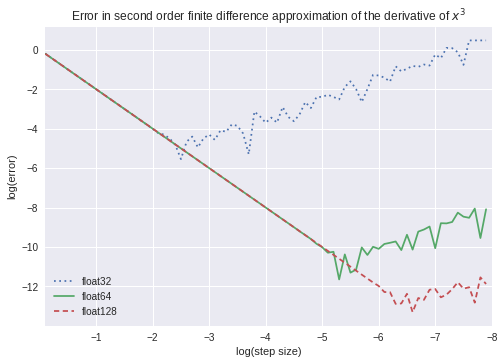
\includegraphics[width=\textwidth]{images/x^3_error_order2.png}
    \caption{This plot show error of using finite difference to approximate the derivative of $x^3$ vs the step size. Observe that the error falls almost linearly until the floating point errors start to dominate, after which it starts to grow erratically. Also, observe that for reasonable step sizes the error falls along a line with slope 2 which is to be expected of a second order approximation. }\label{fig:x^3_error_order2}
    \index{figures}
\end{figure}


To give some perspective, while solving the scalar collapse equations we are going to use step size of the order $10^{-5}$, thus using float32 is just out of the picture. Which implies that there will be at least $10^{5}$ operations per element (we can not decrease spatial step size without decreasing the time step size at the same time, something we will explore more in the next sections). From the discussion in the section \ref{para:addition_errors} we know that there is an error associated with each operation as well, thus even though individual errors may be small but given the size of calculations we are interested in they can quickly add up and destroy our simulations.





Having discussed the effect of the step size on the error of finite difference method we now turn to another major source of error. While talking about the error in the equation \ref{eq:1d_1o_error} we conveniently ignored the dependence of the error on the second derivative $y''(x_0)$. One can ask what will happen if the second derivative is itself very larger?

This is the question that  try to answer. We know that,

\begin{equation}
    \frac{d^n}{dx^n}\left(\frac{1}{x}\right) = (-1)^n \frac{n!}{x^(n+1)}
\end{equation}

Because the derivatives are themselves very larger close to the origin the error in our finite difference approximation keeps on increasing with as we get closer to the origin. This can be seen in the figures \ref{fig:1/x_1}, \ref{fig:1/x_0.1}, \ref{fig:1/x_0.01}. Notice how we have to take smaller and smaller step size to get the same accuracy as we get closer to the origin.

The approximation at $x=0.01$ is so bad that even taking the step size to be $10^{-10}$ is not giving very accurate answer (Figure \ref{fig:1/x_0.01}.

\textbf{The crux of the matter is that first order finite difference methods struggle when the functions is changing very fast}. Something we will see in the results of our simulations.


\begin{figure}[hbt!]
    \centering
    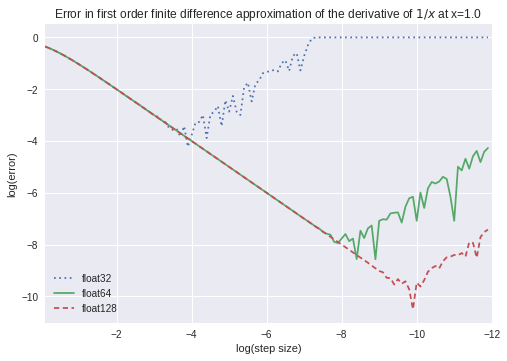
\includegraphics[width=0.8\textwidth]{images/1_x_error_at_1.png}
    \caption{This plot show error of using finite difference to approximate the derivative of $\frac{1}{x}$ vs the step size at $x = 1$.}
    \label{fig:1/x_1}
    \index{figures}
\end{figure}

\begin{figure}[hbt!]
    \centering
    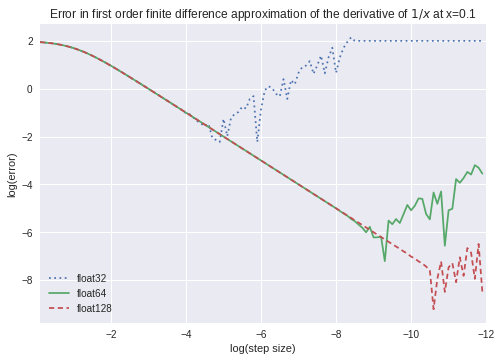
\includegraphics[width=0.8\textwidth]{images/1_x_error_at_p1.png}
    \caption{This plot show error of using finite difference to approximate the derivative of $\frac{1}{x}$ vs the step size at $x = 0.1$.}
    \label{fig:1/x_0.1}
    \index{figures}
\end{figure}


\begin{figure}[hbt!]
    \centering
    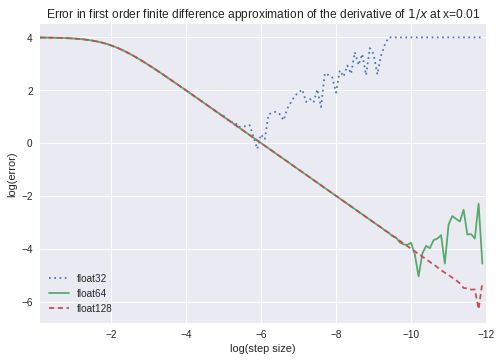
\includegraphics[width=0.8\textwidth]{images/1_x_error_at_p01.png}
    \caption{This plot show error of using finite difference to approximate the derivative of $\frac{1}{x}$ vs the step size at $x = 0.01$.}
    \label{fig:1/x_0.01}
    \index{figures}
\end{figure}


Although, this situation is still salvageable by using higher order methods as shown in the Figure \ref{fig:1/x_error_vs_order}. Notice that for the same step size the higher order methods are much more accurate, just by going to second order methods we are able to reduce the errors by a lot. Furthermore, using even higher order methods gives a diminishing return which is one of the reasons why we will be using second order methods.

\begin{figure}[hbt!]
    \centering
    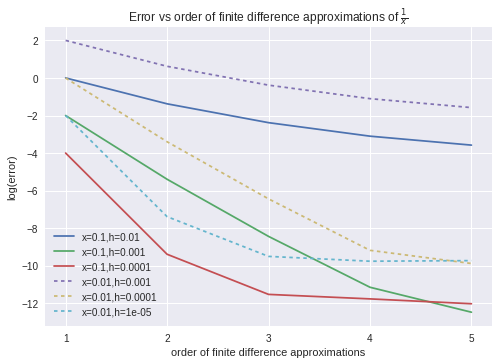
\includegraphics[width=\textwidth]{images/1_x_error_vs_order.png}
    \caption{This plot show error of using finite difference to approximate the derivative of $\frac{1}{x}$ vs the order of the approximation.}
    \label{fig:1/x_error_vs_order}
    \index{figures}
\end{figure}